\chapter{Αποτελέσματα}
Στο παρόν κεφάλαιο παρουσιάζονται τα αποτελέσματα από το μοντέλο βελτιστοποίησης της λειτουργίας του υπό μελέτη μικροδικτύου, βάσει του συνολικού κόστους λειτουργίας του.
Μελετώνται και οι δύο καταστάσεις του μικροδικτύου, σύνδεσης στο κεντρικό δίκτυο, αλλά και νησιδοποίησης. Σε κάθε κατάσταση μελετώνται διάφορα σενάρια προσφοράς και ζήτησης ενέργειας. Ενώ στην κατάσταση σύνδεσης στο κεντρικό δίκτυο δίνεται ιδαίτερη προσοχή και στην τιμή αγοράς και πώλησης της ενέργειας. 

\en
\section{Islanded}
Παρακάτω παρουσιάζονται διάφορα σενάρια της βελτιστοποίησης του υπό μελέτη μικροδικτύου όταν αυτό βρίσκεται σε κατάσταση νησιδοποίησης. 

\gr
\subsection{Τυπική ημέρα Καλοκαιριού}
Περίσσεια ενέργειας από το φωτοβολταϊκό σύστημα. 

\begin{figure}[H]  % 'H' forces the figure to stay exactly where it is placed
    \centering
    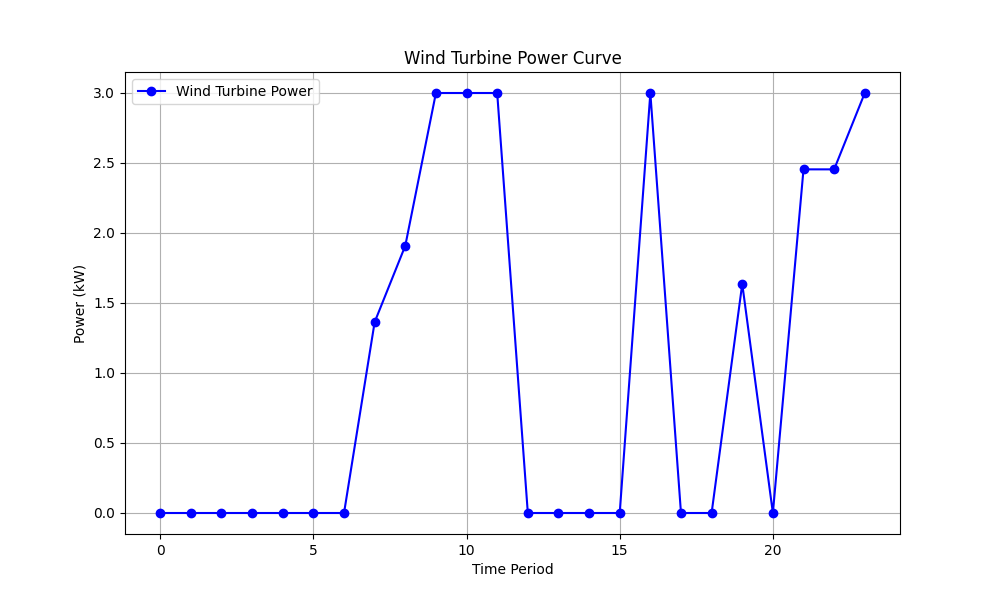
\includegraphics[width=0.8\textwidth]{figures/Figure_2.png}  % Adjust the width as needed
    \caption{Καμπύλη Ισχύος Ανεμογεννήτριας}
    \label{fig:my_label}
\end{figure}

\begin{figure}[H]  % 'H' forces the figure to stay exactly where it is placed
    \centering
    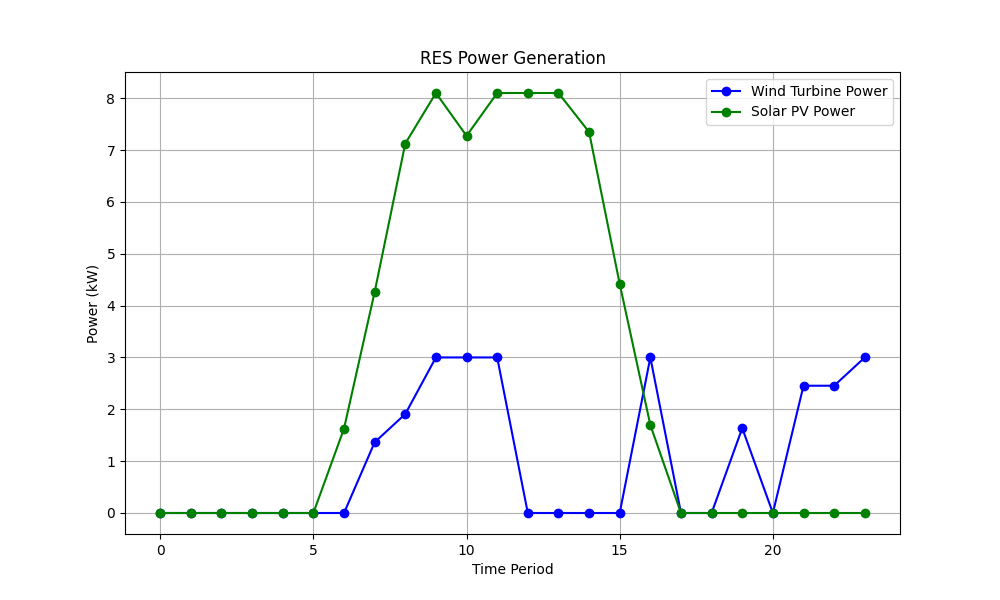
\includegraphics[width=0.8\textwidth]{figures/Figure_3.png}  % Adjust the width as needed
    \caption{Καμπύλη Ισχύος Ανανεώσιμων}
    \label{fig:my_label}
\end{figure}

Παρατηρείται ότι η παραγωγή ενέργειας κατά τη διάρκεια της ημέρας προκύπτει από τις δύο μονάδες ανανεώσιμων πηγών ενέργειας του μικροδικτύου, το σύστημα φωτοβολταϊκών πάνελ και την ανεμογεννήτρια. Η καμπύλη φορτίου ακολουθεί μία τυπική μορφή, με δύο μέγιστα. Ένα μέγιστο κατά τις πρωινές ώρες και ένα μεγαλύτερο κατά τις βραδινές ώρες. Φαίνεται πως η ισχύς που παράγεται από τα φωτοβολταϊκά πάνελ είναι σημαντικά μεγαλύτερη της ανεμογεννήτριας, γεγονός που υποδεικνύει ότι στο σύστημα θα υπάρχει περίσσεια ενέργειας, η οποία θα πρέπει να διοχετευθεί στις μονάδες αποθήκευσης. 

\begin{figure}[H]  % 'H' forces the figure to stay exactly where it is placed
    \centering
    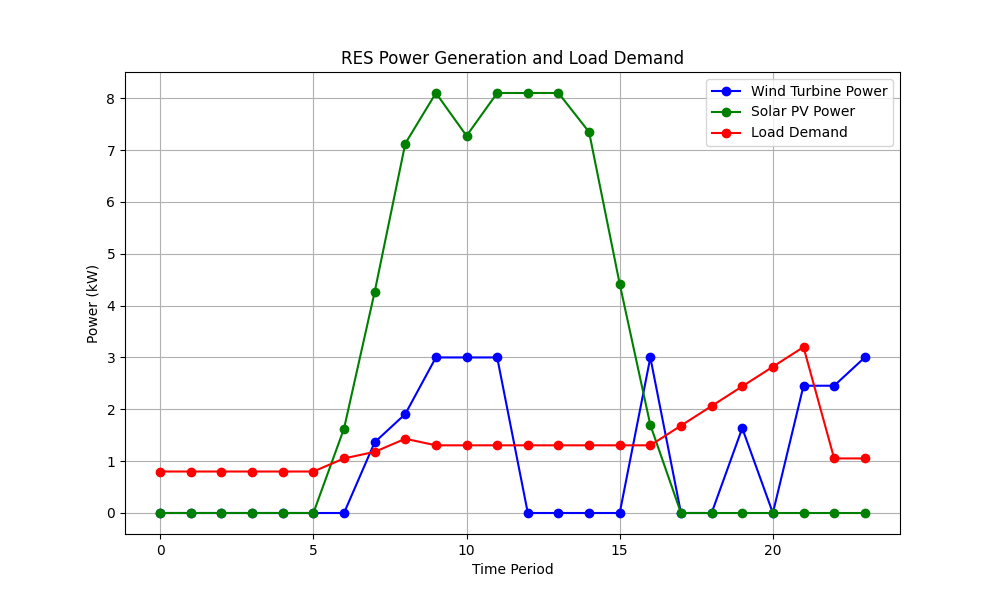
\includegraphics[width=0.8\textwidth]{figures/Figure_4.png}  % Adjust the width as needed
    \caption{Καμπύλη Παραγωγής και Καμπύλη φορτίου}
    \label{fig:my_label}
\end{figure}


\begin{figure}[H]  % 'H' forces the figure to stay exactly where it is placed
    \centering
    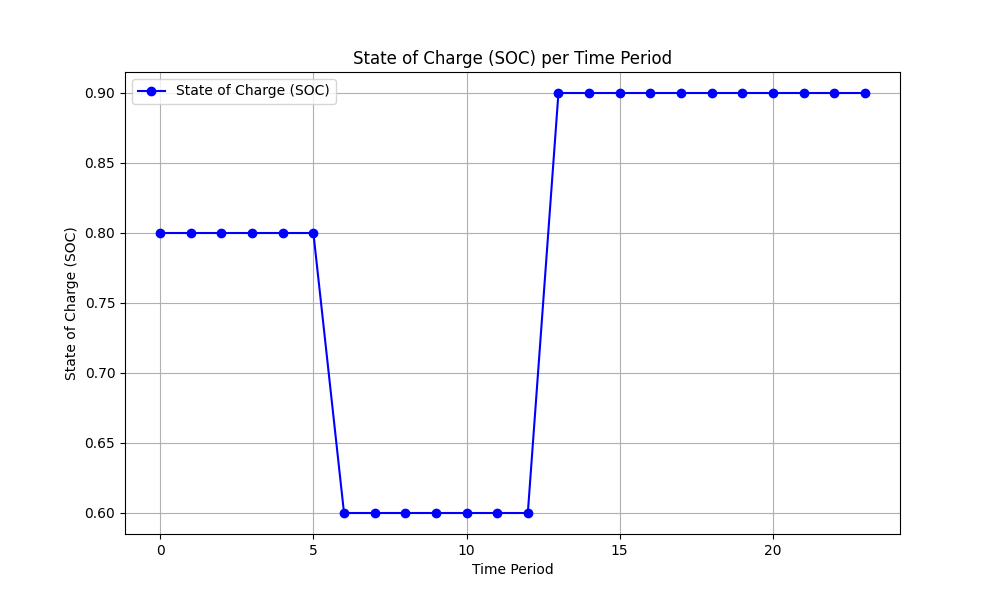
\includegraphics[width=0.8\textwidth]{figures/Figure_5.png}  % Adjust the width as needed
    \caption{Κατάσταση φόρτισης μονάδας μπαταριών}
    \label{fig:my_label}
\end{figure}

\begin{figure}[H]  % 'H' forces the figure to stay exactly where it is placed
    \centering
    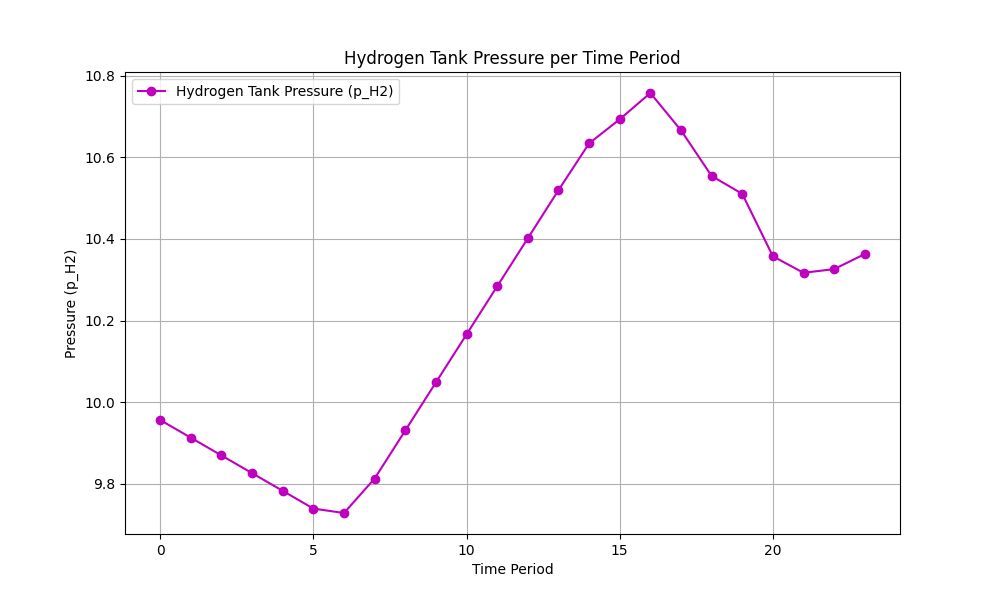
\includegraphics[width=0.8\textwidth]{figures/Figure_6.png}  % Adjust the width as needed
    \caption{Πίεση Δεξαμενής Υδρογόνου}
    \label{fig:my_label}
\end{figure}

\begin{figure}[H]  % 'H' forces the figure to stay exactly where it is placed
    \centering
    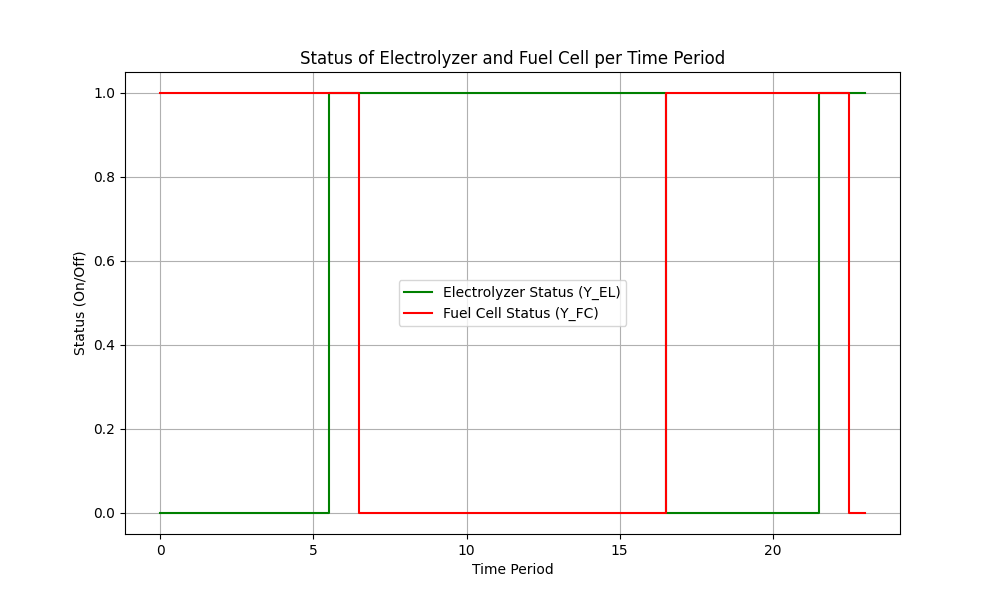
\includegraphics[width=0.8\textwidth]{figures/Figure_7.png}  % Adjust the width as needed
    \caption{Κατάσταση λειτουργίας μονάδας υδρογόνου}
    \label{fig:my_label}
\end{figure}

\subsection{Τυπική ημέρα Φθινοπώρου}
\subsection{Τυπική ημέρα Χειμώνα}
\subsection{Τυπική ημέρα Άνοιξης}

\subsection{Ειδικές περιπτώσεις}
\subsubsection{Αστοχία Μονάδων Παραγωγής}

\en
\section{Grid-connected}

\gr